% Capítulo 3
\chapter{Revisão do Estado da Arte}
\label{cap:cap3}

Este capítulo busca compreender o estado da arte e identificar desafios e oportunidades de pesquisa sobre a implementação de mecanismo \textit{throttling}, especialmente no contexto de dispositivos \acs{IoT} presentes na computação dirigia à energia (\acl{EDC}). Assim, foi realizado uma pesquisa sobre a aplicação de fatores limitantes e os motivadores da atuação desse mecanismo.


\section{Protocolo}
Para esta revisão, adotaram-se práticas descritas no método apresentado por \citeauthor{kitchenham_systematic_2009} (\citeyear{kitchenham_systematic_2009}), mas decidiu-se por não utilizar uma revisão sistemática como protocolo. Assim, a captação dos estudos foi realizada através da aplicação da técnica de \textit{snowballing}, que é capaz de expandir a base de referências e viabilizar a identificação de padrões recorrentes, aprofundando a compreensão no tema de estudo.

O processo de \textit{snowballing} é descrito como abordagem iterativa de busca por referências em revisões de literatura \cite{wohlin_guidelines_2014}. Seu método é caracterizado através das iterações onde em cada uma é realizado análise sobre as referencias citadas nos artigos seminais (\textit{backward}) e também dos estudos que utilizaram esses artigos como referencia (\textit{forward}). Portanto, neste trabalho a abordagem de \textit{snowballing} foi executada em iterações, aplicando ambos os métodos (\textit{backward} e \textit{forward}). Os trabalhos resultantes de cada iteração  foram incluídos com base nos critérios de seleção previamente definidos na Subseção \ref{cap3:criteriosinclusaoexclusao}.


\subsection{Critérios de inclusão e exclusão} 
\label{cap3:criteriosinclusaoexclusao}

Tendo em vista a necessidade de realizar filtragem no material encontrado durante iterações, foram adotados critérios de inclusão e exclusão como já previsto no método em  \cite{wohlin_guidelines_2014}. Assim, os estudos resultantes foram obtidos com base nos critérios definidos com a intenção de cobrir o maior numero de trabalhos relacionados ao tema de pesquisa e ao mesmo tempo evitar os trabalhos com base nos critérios estabelecidos.

Portanto, os critérios de exclusão utilizados podem ser vistos descritivamente na Tabela \ref{table:cap3:criterios}. Estes critérios foram definidos para assegurar que apenas os estudos que se relacionassem com a pesquisa fossem incluídos, evitando artigos segundo os critérios ja apresentados.


\begingroup
\begin{table}[htbp]
	
	\centering
	\caption{\textit{Snowballilng}: Critérios de Exclusão.}
	%	\small
	%	\tabcolsep=0.05cm
	\begin{tabular}{ l | l  }
		\hline
		 \multicolumn{2}{c}{Critério de Exclusão}  \\
		\hline\addlinespace[1pt]
		CE-1	& Não escrito em inglês. \\
      	CE-2	& Sem aderência aos eixos temáticos. \\
		CE-3	& Sem indícios diretos com às questões de pesquisa.\\
		CE-4	& Artigos derivações do mesmo autor  ou resumo.\\
		CE-5	& Tutoriais, Capítulos de livros e Relatórios técnicos (Literatura Cinza).\\
		CE-6	& Trabalhos duplicados.\\
		CE-7	& Artigos não disponíveis integralmente para leitura.\\
		CE-8	&  Artigos predecessores à revisão seminal.\\
		\hline\addlinespace[2pt]
	\end{tabular}
	\label{table:cap3:criterios}
	\\
	\footnotesize Fonte: elaborado pelo autor.
	
\end{table}
\endgroup

\subsection{Processo}

Para selecionar os estudos que formam a base do trabalho foi utilizada a base bibliográfica SciVerse Scopus
\footnote{Plataforma acessível em: \url{https://www.scopus.com/}}. A escolha desta plataforma como fonte de informação foi justificada pela capacidade de indexar os principais repositórios acadêmicos para a area de estudo, dentre elas ACM Digital Library, Elsevier, IEEE Xplore, Springer Link, Web of Science entre outras.

O artigo seminal foi selecionado mediante análise de sua influência, impacto e credibilidade para o campo de pesquisa deste estudo. Portanto, utilizando o artigo como único ponto de partida, segue o processo iterativo \textit{snowballing} conforme estabelecido. As etapas podem ser visualizadas na Figura \ref{fig:cap3snowballing} onde é apresentado a visão completa do processo e ações determinadas.


\begin{figure}[H]
	\centering	
	\caption{Processo \textit{Snowballing}.} 
	\label{fig:cap3snowballing}
	\noindent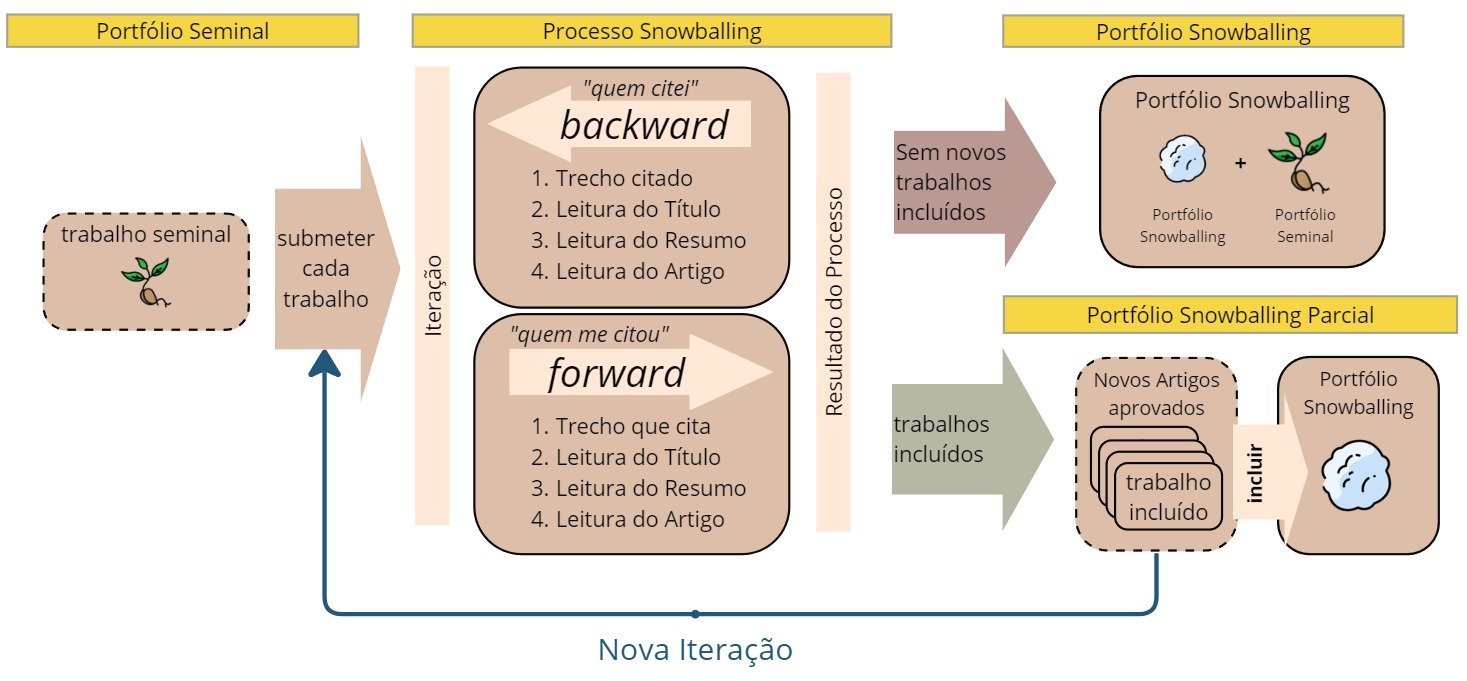
\includegraphics[width=1\linewidth]{Imagens/cap3/snowballing.jpg} 
	
	Fonte: elaborado pelo autor.
\end{figure}

Em cada iteração, são realizadas ações com o objetivo de selecionar os trabalhos considerados relevantes para o estudo. Essas, partem da análise da leitura da parte do texto que foi citado quando em \textit{backward} ou a leitura do trecho que cita quando em \textit{forward}, além da leitura do titulo, resumo e por fim, da leitura integral do trabalho. Assim, ao passo que finalizada interação, teremos os novos artigos que servem como entrada para iteração seguinte. Caso uma iteração finalize sem nenhum novo trabalho adicionado, conclui-se o processo \textit{snowballing}, os resultados são unidos ao artigo seminal em composição ao portfólio final obtido. A Figura \ref{fig:cap3etapassnowballing} apresenta o processo de seleção dos trabalhos avaliados.

\begin{figure}[H]
	\centering	
	\caption{Resultado das Iterações \textit{Snowballing}.} 
	\label{fig:cap3etapassnowballing}
	\noindent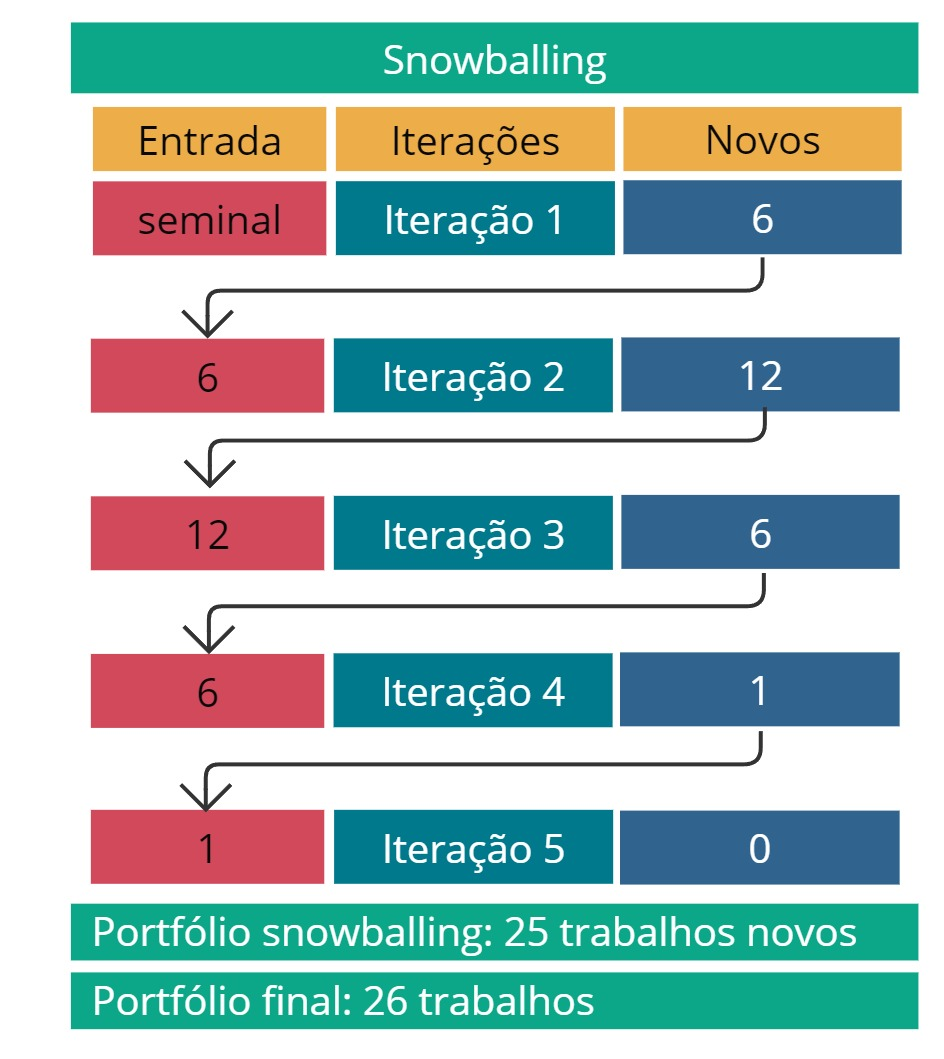
\includegraphics[width=0.7\linewidth]{Imagens/cap3/etapas.jpg} 
	
	Fonte: elaborado pelo autor.
\end{figure}


A dinâmica de inclusão e filtragem de trabalhos relacionados, proporcionou visitar ao todo 1132 trabalhos por método \textit{backward}, além de 3582 trabalhos por \textit{forward} gerando uma cobertura total de 4714 artigos alcançados. É previsto durante o \textit{snowballing} proporcionar rastreabilidade na inclusão dos trabalhos. A Figura apresenta esta característica enquanto proporciona visão sobre os trabalhos mencionados. 

\begin{figure}[H]
	\centering	
	\caption{PENSANDO SE VALE APRESENTAR GRAFO COM A a rastreabilidade dos trabalhos aqui.} 
	\label{fig:cap3etapassnowballing}
	\noindent\includegraphics[width=0.7\linewidth]{example-image} 
	
	Fonte: elaborado pelo autor.
\end{figure}

Finalmente o processo Snowballing proporcionou a criação do portfólio total de artigos, composto por 25 trabalhos que serviram como base para o estudo, os resultados obtidos estão descritos na Seção \ref{cap3:resultados}.


\section{Resultados}
\label{cap3:resultados}

Foi característica do portfólio de trabalhos a apresentação dos desafios enfrentados pelos agentes \acs{IoT} com capacidade de coleta de energia ao realizar suas funções, mesmo diante de restrições energéticas. Nestes trabalhos, foi observada a presença de mecanismos de ajuste do comportamento que utilizam observações de determinadas variáveis para tomar decisões sobre como o dispositivo deve conduzir seus ciclos em diferentes cenários.

Sendo assim, mediante desafios apresentados nos estudos quanto à gestão energética desses dispositivos, foi considerado categorizar dos trabalhos em função dos grupos definidos no estudo \cite{khan_energy_2015}. Por análise de atuação orientada à dados, os trabalhos apresentam a possibilidade de atividades em respeito a previsibilidade dos dados de coleta e demanda energética. Assim, a categorização puramente baseada nos ciclos (\textit{Duty-Cycle}) do dispositivo carregam os fatores de observação atrelados as aspectos energéticos de coleta e armazenamento como motivadores para ajustes no tempo de ciclos ou ocorrência destes para adaptar-se aos critérios de energéticos impostos.

Portanto, diante dos desafios identificados nos estudos sobre a gestão energética desses dispositivos, optou-se por categorizá-los com base nos grupos definidos no estudo realizado por \cite{khan_energy_2015}. Nesse contexto, um grupo de trabalhos se concentram aos desafios de definir os ciclos de operação observando eventos relacionados aos aspectos energéticos de coleta e armazenamento respectivamente. Por sua vez, ao abordar o processo de definir seus ciclos, alguns estudos apontam avanços em tecnicas que buscam prever o comportamento do dispositivo, em especial sua demanda e capacidade de coleta de energia. 

Em última análise, todos os esforços convergem para a análise de como os estudos moldam o escopo decisório da ação do agente limitador (\textit{throttling}) sobre seus ciclos. Além disso, o portfólio alcançado inclui cinco trabalhos categorizados como filosóficos, caracterizados pela apresentação de contribuições puramente conceituais. Esses trabalhos se concentram na análise teórica dos problemas relacionados à computação voltada para a energia, sem necessariamente fornecer implementações práticas, o que se alinha ao modelo de categorização proposto por \citeonline{Wieringa2006}.


Um ponto de destaque é que, à primeira vista, pode-se imaginar menor necessidade da presença dos mecanismos limitantes, especialmente onde dispositivo esta preparado para realizar operações transientes. No entanto, apesar da característica energética, ainda persiste necessidade de mecanismos limitadores, desde que o dispositivo tenha por objetivo operar seus ciclos de forma parcial, motivado pelo iminente esgotamento energético (\cite{merrett_energy-driven_2017}; \cite{sliper_energy-driven_2020}).

\begin{figure}[H]
	\centering	
	\caption{Categorização dos Trabalhos} 
	\label{fig:cap3:divisaodosestudos}
	\noindent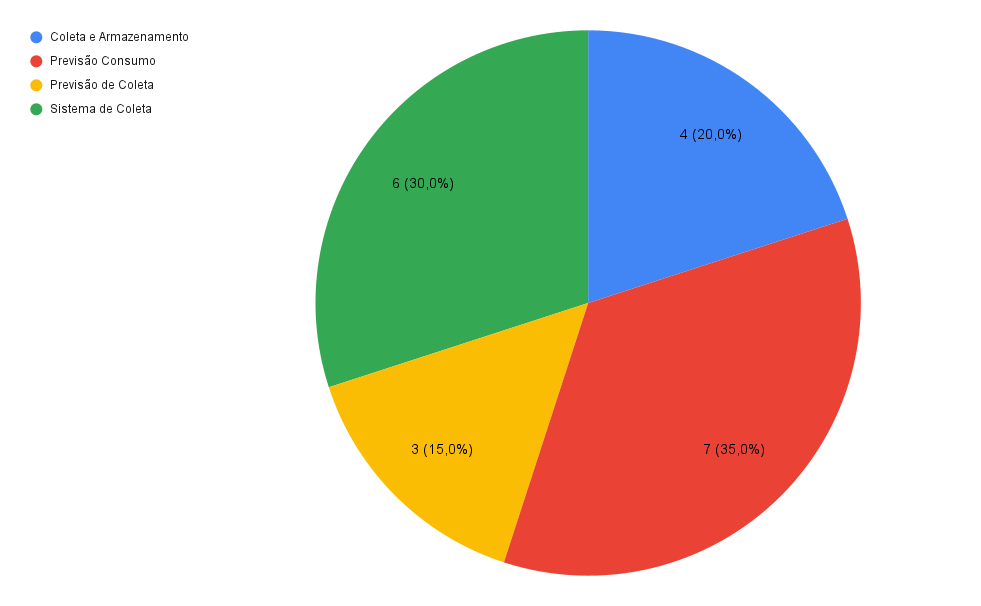
\includegraphics[width=0.8\linewidth]{Imagens/cap3/classificacao.png} 
	
	Fonte: elaborado pelo autor.
\end{figure}


Devido à necessidade de caracterizar as operações realizadas pelos dispositivos, há uma uniformidade quanto ao uso do termo "ciclo" (\textit{Duty-Cycle}) quando se pretende fazer referência às janelas de operação, nas quais o dispositivo realizará as atividades a que se propõe. Mesmo os trabalhos categorizados como soluções orientadas previsão  conforme visto na categorização apresentada na Figura \ref{fig:cap3:divisaodosestudos} apoiam-se na definição proposta por \citeonline{kansal_power_2007}, que trata ciclos como a referencia do tempo de duração das atividades que induzem um dispositivo à mudança de estados e, por sua vez, requerem capacidade energética (\citeonline{jaber_reducing_2017}; \citeonline{shen_energy-efficient_2019}; \citeonline{balsamo_hibernus_2016}; \citeonline{lee_energy_2018}). 

As soluções e propostas de adaptação dos ciclos podem ser categorizadas da seguinte forma: Primeiramente, destacam-se as abordagens que se concentram nos desafios relacionados à coleta de energia e, como consequência desses eventos, propõem mecanismos de controle e ajustes orientados a capacidade de coleta. Por exemplo, \citeonline{doumenis_lightweight_2022} descreve uma análise sobre o balanço energético coletado para definir a utilização energética do ciclo. Por outro lado, (\citeonline{choi_adaptive_2020}; \citeonline{balsamo_graceful_2016}; \citeonline{khairnar_discrete-rate_2015};) exploram, a partir da performance instantânea dos sistemas de coleta, a descoberta de motivadores para modelar a atuação do agente limitante, buscando ciclos com características neutro-potenciais.


Apesar de não se concentrar em uma solução especifica, \citeonline{kansal_power_2007} apresentam os conceitos fundamentais da teoria de coleta de energia, determinante para computação dirigida à energia. No estudo realizados por (\citeonline{khairnar_power_2011}; \citeonline{sudevalayam_energy_2011}) é considerada a possibilidade de incorporar um componente de armazenamento intermediário em conjunto com as analises de coleta, para definir como o agente limitante irá agir sobre os ciclos. Nesta direção, a proposta de \citeonline{yoo_dynamic_2012} busca comparar os valores de coleta e armazenamento para estimar como deverá ser o comportamento do dispositivo nos ciclos futuros.

Para \citeonline{liu_energy_2016}, a solução apresentada considera os custos de transmissão para definir o gasto energético durante os ciclos e assim decidir como operará. Em (\citeonline{ge_adaptive_2020};\citeonline{arnaiz_energy_2024}) é utilizado técnicas de aprendizado de máquina em busca de prever coleta e consumo de energia respectivamente. Ambos buscam antecipar características energéticas vindouras, bem como demandas ao passo que podem adaptar-se suavemente até alcançar patamar pretendido.

Outra abordagem encontrada é a desativação de recursos conforme necessário, como apresentado por \citeonline{shen_energy-efficient_2019}. Durante os ciclos, os dispositivos podem reduzir ou desligar o consumo energético de componentes não essenciais, entrando em modo restrito para reduzir o uso de energia e se adequar aos valores armazenados. Em (\citeonline{zhang_toward_2018}; \citeonline{gong_sleep_2022}), são utilizados os processos estatísticos como tomadores de decisão, baseadas em uma certa previsibilidade no fornecimento de energia e favorecido pelas características de noção do ambiente \textit{Context-Awareness} em que o dispositivo \acs{IoT} se encontra. Finalmente, a Tabela \ref{table:cap3:solucoesparajaneladeoperacoes} apresenta um resumo dos contextos nos quais o agente limitador utiliza como motivador para atuar sobre a dinâmica dos ciclos no dispositivo.


\begin{table}[H]
	\centering
	\caption{Estratégias definidoras dos ciclos de operação.}
	\small
	\rowcolors{1}{gray!10}{white}
	\begin{tabularx}{\textwidth}{|X|X|}
		\hline
		\textbf{Baseado em} &\textbf{Referência} \\
		\hline
		\multirow{6}{*}{Sistema de Coleta} & \citeonline{choi_adaptive_2020}  \\
		& \citeonline{balsamo_graceful_2016} \\
				&\citeonline{balsamo_hibernus_2016}\\
					&	\citeonline{khairnar_discrete-rate_2015} \\

		&\citeonline{benhamaid_recent_2022} \\
		&\citeonline{doumenis_lightweight_2022}\\

		\hline
		\multirow{4}{*}{Sistema de Coleta e Status Armazenamento} & \citeonline{kansal_power_2007}\\
			& \citeonline{khairnar_power_2011} \\
		&	\citeonline{sudevalayam_energy_2011} \\
		&   \citeonline{yoo_dynamic_2012}\\
		\hline
		\multirow{3}{*}{Previsão de coleta} &\citeonline{ge_adaptive_2020}\\
			&	\citeonline{zhang_toward_2018}\\
			&	\citeonline{gong_sleep_2022}\\
		\hline
		\multirow{7}{*}{Previsão de consumo} & \citeonline{arnaiz_energy_2024}\\		
			& \citeonline{lee_energy_2018}\\
			& \citeonline{luo_optimal_2017} \\
			& \citeonline{liu_energy_2016}\\
			& \citeonline{liu_performance_2015}\\
			& \citeonline{jaber_reducing_2017}\\
			& \citeonline{shen_energy-efficient_2019}\\
			\hline
		
		
		
	\end{tabularx}
	\label{table:cap3:solucoesparajaneladeoperacoes}
	
	Fonte: Elaborado pelo autor.
\end{table}

Ao analisar as características dos dispositivos \acs{IoT} que operam em restrições energéticas, a atuação dos mecanismos limitantes e as estratégias utilizadas para definir seus ciclos de operação, surge a necessidade de uma organização sistematizada dos fatores apresentados. Essa organização em formato taxonômico permite identificar e classificar os diversos aspectos que influenciam e demandam atenção na implementação do throttling, uma alternativa no processo de controle do comportamento durante os ciclos dos dispositivos.


Finalmente, a criação de taxonomia adequada possibilita uma compreensão clara das diferentes variáveis envolvidas, como características dos dispositivos, atividades realizadas, demandas de energia e estratégias de atuação do \textit{throttling}. Isso permitiria uma abordagem mais sistemática na implementação do padrão, garantindo uma gestão eficaz dos recursos energéticos o que favorece o incremento de disponibilidade enquanto conserva suas capacidades energéticas.


%\blindtext[2]